\subsection{Winkelverteilung}
\subsubsection{Schwellenkurve}
Bevor man die Winkelverteilung messen kann, muss zuerst die optimale Schwelle für den Diskriminator D12 bestimmt werden. Dazu wird die Schwelle des Diskrimators von -50 bis -250 \si{\milli\volt} in 10 \si{\milli\volt} Schritten verändert und jeweils für 2520 \si{\second} die Anzahl der Koinzidenzen von D12 mit D23, D24, D1 oder D2 gemessen. Dies wird über ein LabVIEW-Programm automatisiert (siehe Abb. \ref{fig:prog_all}).\\

\begin{figure}
\centering
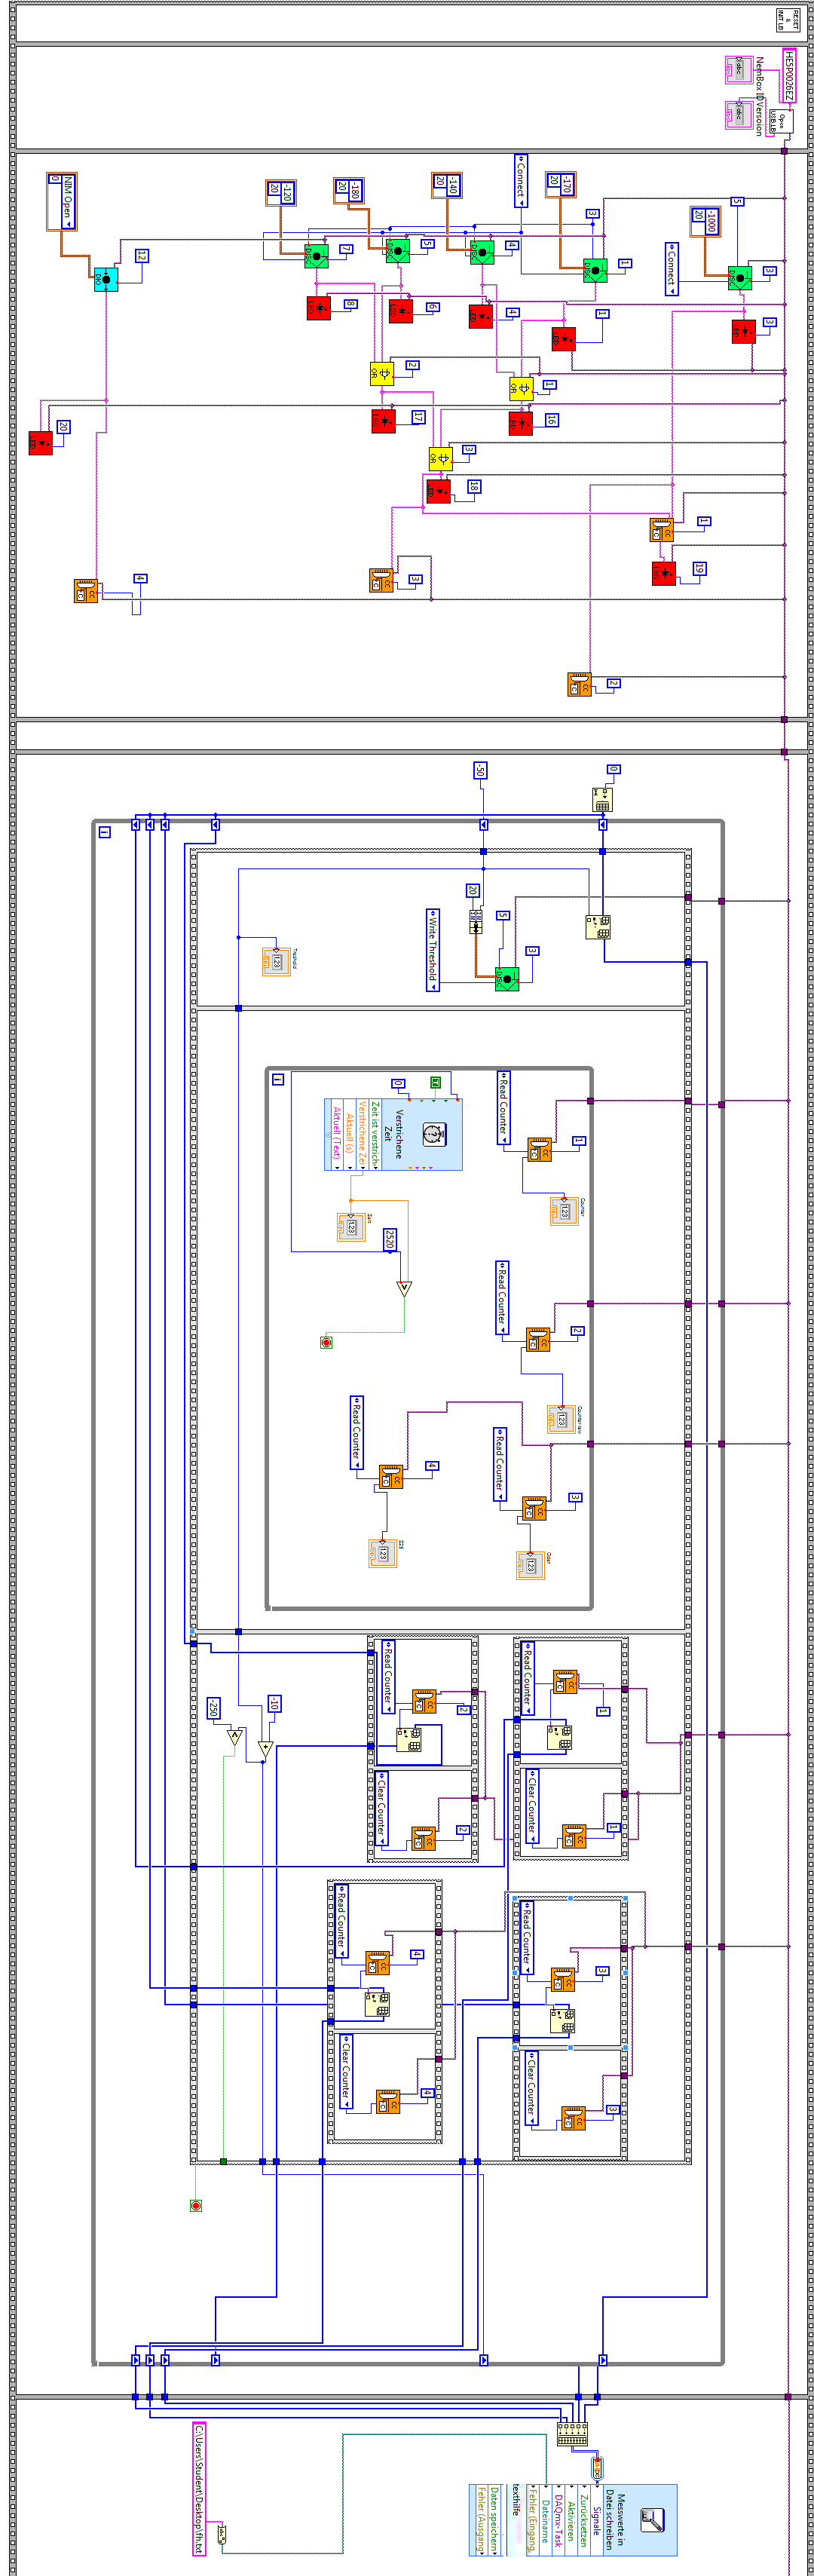
\includegraphics[height=20cm]{data/friedrich/prog_ges_rot.png}
\caption{Gesamtes Programm}
\label{fig:prog_all}
\end{figure}

Im ersten Teil des Programmes wird die Hardware initialisiert (siehe Abb. \ref{fig:prog_init}). Im wesentlichen werden die Diskrimatoren D12 (Id 3), D23, D24, D1, D2 (Ids 1, 4, 5, 7) und D25 (Id 7) mit einer LED verbunden. Danach wird das ODER-Signal aus den Signalen D23, D24, D1 und D2 ermittelt, indem man sie über Oder-Blöcke verknüpft. Das Ausgangssignal wird wieder auf eine LED gegeben. Um Signale zu zählen werden Koinzidenzzähler verwendet. Zähler 1 zählt Koinzidenzen aus D12 und dem ODER-Signal, Zähler 2 die Anzahl der Signale in D12, Zähler 3 die ODER-Signale und Zähler 4 die Signale aus D25. \\
 
\begin{figure}
\centering
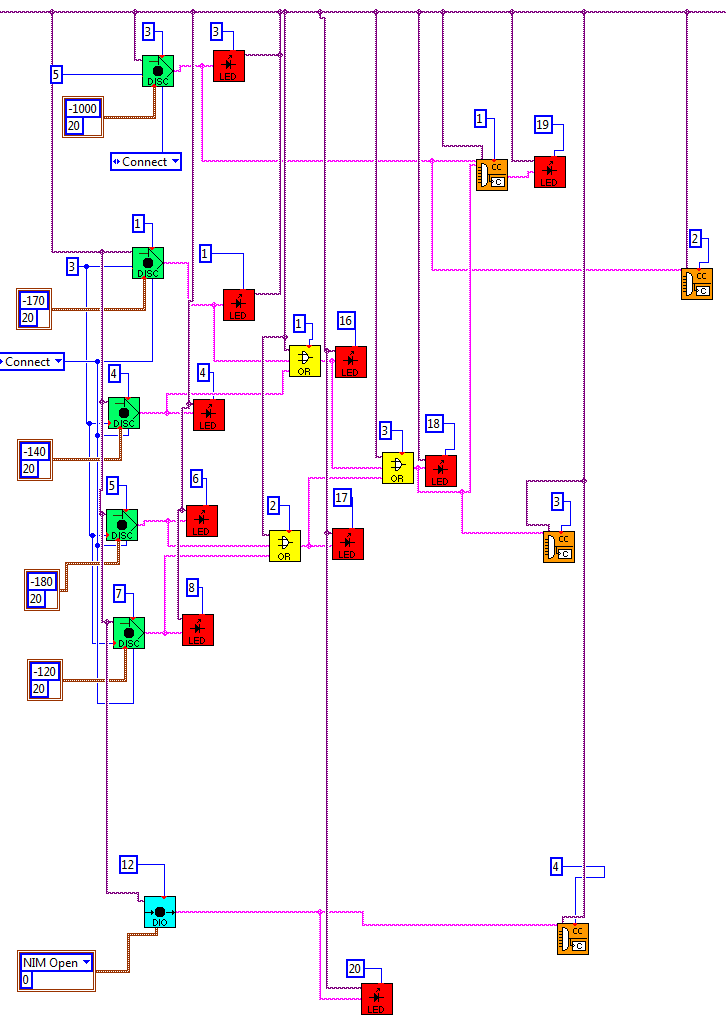
\includegraphics[height=20cm]{data/friedrich/prog_init.png}
\caption{Hardwareinitialisierung}
\label{fig:prog_init}
\end{figure}

Der zweite Teil besteht aus zwei verschachtelten Schleifen (siehe Abb. \ref{fig:prog_prog}). Vor der äußeren Schleife wird die Schwelle auf einen Startwert gesetzt (-50\si{\milli\volt}) und fünf Arrays initialisiert (eines, um die Schwellenwerte zu speichern und die anderen vier für die Anzahl der Ereignisse in den Koinzidenzzählern). Die äußere Schleife setzt den Schwellenwert des Diskriminators und speichert ihn im Array, wartet dann 2520\si{\second} und fügt dann die gemessenen Koinzidenzen der einzelnen Koinzidenzzähler an die jeweiligen Arrays ein. Danach werden die Zähler zurückgesetzt und die Schwelle um 10 \si{\milli\volt} verringert, bis -250 \si{\milli\volt} erreicht wurden.\\
Die innere Schleife ist im wesentlichen dazu da, um die 2520\si{\second} zu warten. Parallel dazu werden die jeweiligen Zählraten im Interaktionsfenster von LabVIEW angezeigt.\\
Zum Schluss des Programmes werden alle Arrays zusammengefasst und in eine Datei geschrieben.

\begin{figure}
\centering
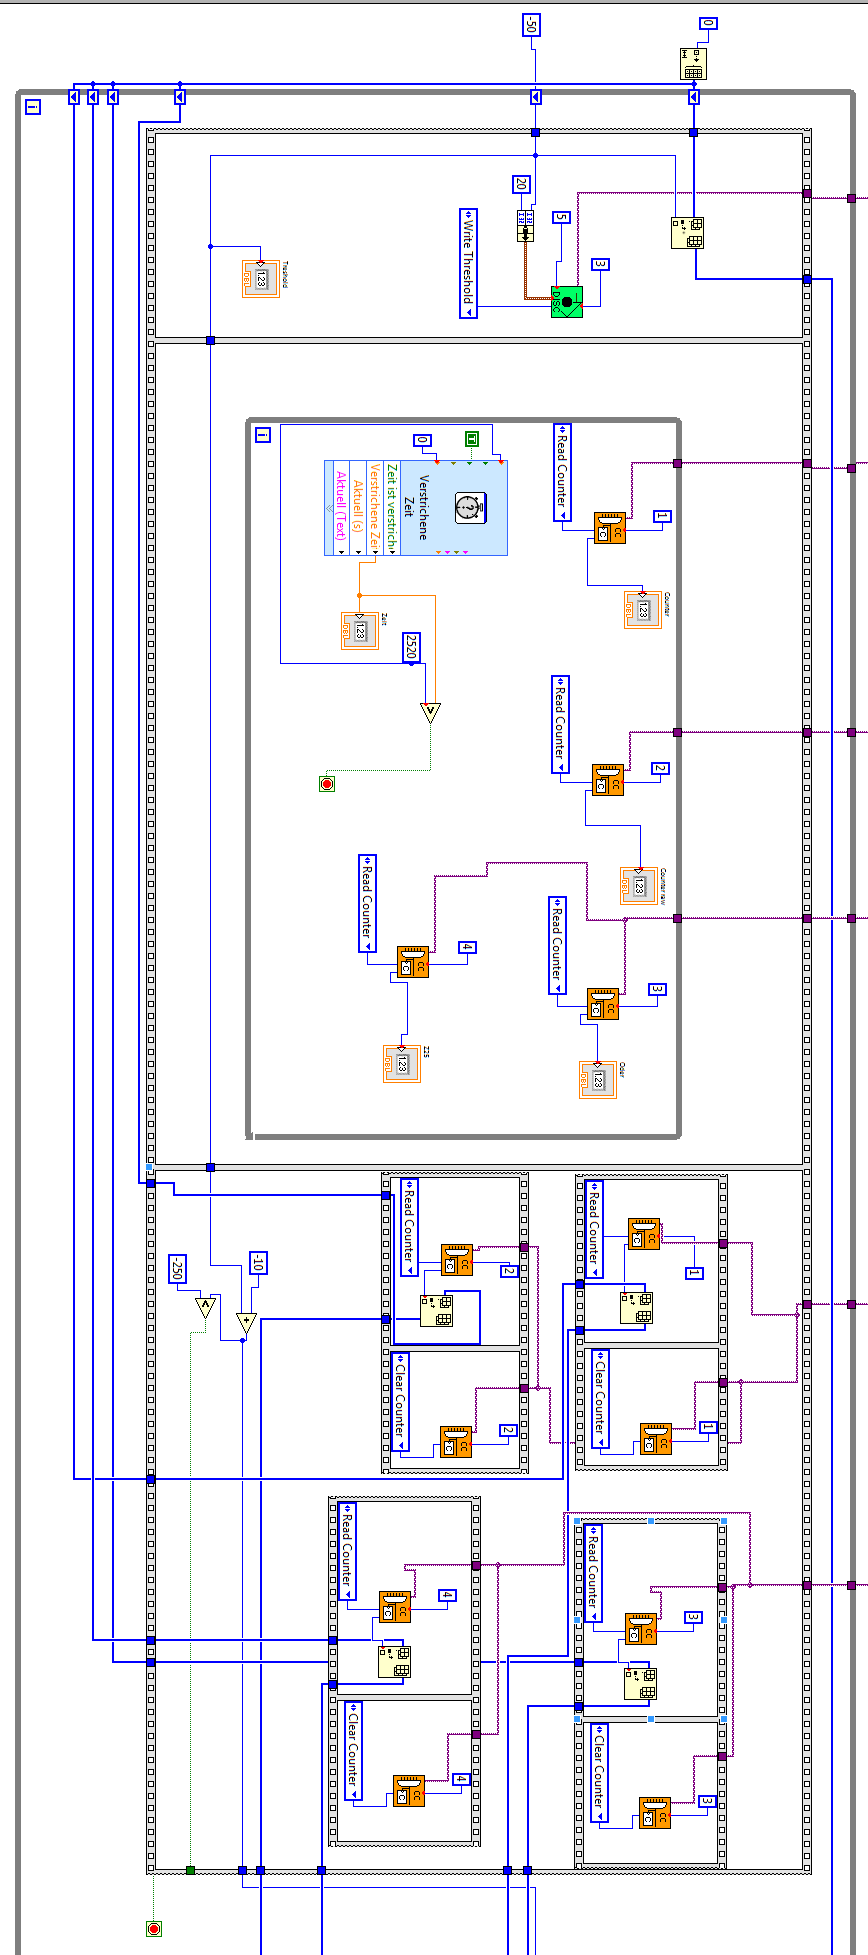
\includegraphics[height=20cm]{data/friedrich/prog_prog_rot.png}
\caption{Hauptprogramm}
\label{fig:prog_prog}
\end{figure}
